\subsection{Input Data}

In the current research on the vehicle routing problems and swarm intelligence, there are some benchmark data available for researchers to use for comparison. However, for the urban transit network design problem (UTNDP), Mandl's network seems to be the only benchmark instance used and acknowledged by researchers, and his work has been widely cited, including \citep{fan09}, \citep{kechagiopoulos14}, \citep{nikolic14}. %Referanser

Christoph Mandl \citep{mandl79} developed a heuristic algorithm for the urban transit network problem. This method was applied and based on a real network in Switzerland, the Swiss transit network\citep{mandl80}. The data includes a small and dense network of 15 nodes and 21 edges, in addition to the travel times and travel demand for each edge. The total demand is 15570 trips per day, which is a relatively high demand for a small network. The travel time between the to farthest nodes in the network is 22 minutes along the shortest path. Mandl developed a solution in two phases, where a feasible set of routes were created in the first phase and in the second phase he tried to minimize the the total travel time, including in-vehicle time and waiting time, by reducing the number of transfers. Some important measures of Mandl's solution network includes, for example, 100\% service coverage, 69.4\% of the trips involving no transfers, 29.93\% of the trips involving one transfer, and only 0.13\% of the trips needing more than one transfer.

We have designed and implemented a method to produce a realistic transit network based on the data from Mandl \citep{mandl79}.The transportation time on each edge is given, and the transportation demand is assumed to be known and constant.  
The data set is downloaded from \citet{mumford13}, which consist of three text files:


\begin{table}[H]
    \begin{center}
        \begin{tabular}{|l|lr|}
     	\hline
     	~ & x & y \\
     	\hline
        1 & 1 & 9 \\
        2 & 3 & 8 \\
        3 & 4.5 & 7.75 \\
        4 & 2.75 & 6.2 \\
        5 & 0.8 & 6.6 \\
        6 & 4.6 & 6 \\
        7 & 7 & 4.5 \\
        8 & 5.5 & 5 \\
        9 & 8.5 & 6.8 \\
        10 & 5.8 & 2.25 \\
        11 & 3.8 & 2.25 \\
        12 & 1.3 & 3.5 \\
    	13 & 5.25 & 1 \\
    	14 & 6.7 & 1.75 \\
    	15 & 6.75 & 5.8 \\
    	\hline
        \end{tabular}
    \end{center}
    \caption {MandlCoordinates.txt}
    \label{table:MandlCoords}
    This file includes 15 lines, with the (x,y) coordinates of the 15 nodes. These coordinates was not supplied in Mandl's literature, so these are copied from \citet{mumford13} and are approximate for the picture to be drawn.
\end{table}


\begin{table}[H]
\resizebox{12.5cm}{!} {
 
    \begin{tabular}{|l|lllllllllllllll|}
    \hline
    ~ & 1       & 2        &  3    &   4     &  5     &  6      & 7      &  8     & 9      & 10      & 11     & 12         &  13     & 14       &  15  \\
    \hline
    1 & 0       & 8        &  Inf    &   Inf     &  Inf     &  Inf      & Inf      &  Inf     & Inf      & Inf      & Inf     & Inf         &  Inf     & Inf       &  Inf  \\
    2 &8       & 0        & 2       &  3        &  6       &  Inf      & Inf      & Inf      & Inf      & Inf      & Inf     & Inf         &  Inf     &  Inf      &  Inf  \\
    3 & Inf     &  2       &  0      &  Inf      & Inf      &  3        &  Inf     &  Inf     & Inf      &  Inf     & Inf     &  Inf        &  Inf     &   Inf     & Inf   \\
    4 & Inf     &  3       &  Inf    &  0        & 4        & 4         & Inf      &  Inf     &  Inf     & Inf      & Inf     & 10          &  Inf     &  Inf      &  Inf  \\
    5 & Inf     &   6      &   Inf   &    4      &   0      & Inf       &  Inf     &  Inf     &   Inf    &   Inf    &    Inf  &     Inf     & Inf      & Inf       & Inf   \\
    6 & Inf     & Inf      &   3     & 4         &  Inf     &  0        &   Inf    &    2     & Inf      & Inf      & Inf     & Inf         & Inf      & Inf       & 3     \\
    7 & Inf     & Inf      &  Inf    &   Inf     &   Inf    &   Inf     & 0        & Inf      &  Inf     &  7       & Inf     & Inf         & Inf      & Inf       &  2    \\
    8 & Inf     & Inf      & Inf     & Inf       & Inf      & 2         & Inf      &  0       &  Inf     &  8       & Inf     &  Inf        &  Inf     & Inf       & 2     \\
    9 & Inf     &  Inf     & Inf     &   Inf     & Inf      & Inf       &  Inf     &  Inf     & 0        &  Inf     & Inf     & Inf         & Inf      & Inf       & 8     \\
    10 & Inf     &  Inf     & Inf     &  Inf      & Inf      &  Inf      & 7        &  8       &  Inf     &  0       & 5       & Inf         & 10       & 8         & Inf   \\
    11 & Inf     &  Inf     & Inf     & Inf       &  Inf     &  Inf      & Inf      & Inf      &  Inf     &   5      & 0       & 10          &  5       & Inf       & Inf   \\
    12 & Inf     & Inf      & Inf     & 10        & Inf      & Inf       & Inf      &  Inf     &  Inf     &  Inf     &  10     & 0           & Inf      & Inf       & Inf   \\
    13 & Inf     & Inf      & Inf     &  Inf      &  Inf     & Inf       &  Inf     &  Inf     &  Inf     & 10       &  5      & Inf         &  0       & 2         &  Inf  \\
    14 & Inf     & Inf      &  Inf    &  Inf      &  Inf     & Inf       &  Inf     & Inf      & Inf      & 8        &  Inf    &  Inf        & 2        & 0         &   Inf \\
    15 & Inf     & Inf      & Inf     & Inf       & Inf      & 3         &  2       &  2       & 8        & Inf      & Inf     &
     Inf         &  Inf     & Inf       &  0    \\
     \hline
    \end{tabular}
}
    \caption {MandlTravelTimes.txt}
    \label{table:MandlTravelTimes}
    The travel times matrix gives the travel times it takes in minutes between the nodes. This matrix is symmetrical, travel times between each node and itself are zero, and ``Inf'' indicates that there is no direct link between the nodes.
\end{table}

\begin{table}[H]
\resizebox{12.5cm}{!} {
 

    \begin{tabular}{|l|lllllllllllllll|}
    \hline
    ~ & 1       & 2        &  3    &   4     &  5     &  6      & 7      &  8     & 9      & 10      & 11     & 12         &  13     & 14       &  15  \\
    \hline
    1 & a   & 400 & 200 & 60  & 80  & 150 & 75  & 75  & 30  & 160 & 30  & 25  & 35  & 0   & 0 \\
    2 & 400 & a   & 50  & 120 & 20  & 180 & 90  & 90  & 15  & 130 & 20  & 10  & 10  & 5   & 0 \\
    3 & 200 & 50  & a   & 40  & 60  & 180 & 90  & 90  & 15  & 45  & 20  & 10  & 10  & 5   & 0 \\
    4 & 60  & 120 & 40  & a   & 50  & 100 & 50  & 50  & 15  & 240 & 40  & 25  & 10  & 5   & 0 \\
    5 & 80  & 20  & 60  & 50  & a   & 50  & 25  & 25  & 10  & 120 & 20  & 15  & 5   & 0   & 0 \\
    6 & 150 & 180 & 180 & 100 & 50  & a   & 100 & 100 & 30  & 880 & 60  & 15  & 15  & 10  & 0 \\
    7 & 75  & 90  & 90  & 50  & 25  & 100 & a   & 50  & 15  & 440 & 35  & 10  & 10  & 5   & 0 \\
    8 & 75  & 90  & 90  & 50  & 25  & 100 & 50  & a   & 15  & 440 & 35  & 10  & 10  & 5   & 0 \\
    9 & 30  & 15  & 15  & 15  & 10  & 30  & 15  & 15  & a   & 140 & 20  & 5   & 0   & 0   & 0 \\
    10 & 160 & 130 & 45  & 240 & 120 & 880 & 440 & 440 & 140 & a   & 600 & 250 & 500 & 200 & 0 \\
    11 & 30  & 20  & 20  & 40  & 20  & 60  & 35  & 35  & 20  & 600 & a   & 75  & 95  & 15  & 0 \\
    12 & 25  & 10  & 10  & 25  & 15  & 15  & 10  & 10  & 5   & 250 & 75  & a   & 70  & 0   & 0 \\
    13 & 35  & 10  & 10  & 10  & 5   & 15  & 10  & 10  & 0   & 500 & 95  & 70  & a   & 45  & 0 \\
    14 & 0   & 5   & 5   & 5   & 0   & 10  & 5   & 5   & 0   & 200 & 15  & 0   & 45  & a   & 0 \\
    15 & 0   & 0   & 0   & 0   & 0   & 0   & 0   & 0   & 0   & 0   & 0   & 0   & 0   & 0   & a \\ 
    \hline
    \end{tabular}
    }
 	\caption {MandlDemand.txt}
 	\label{table:MandlDemand}
 	The demand matrix shows the travel demand between each node pair, which is the average number of passenger trips per day. This matrix is also symmetrical. (These is no demand either to or from node 15, but it there is demand to node 9, which is only connected to node 15). For coding reasons, we changed the numbers in the main diagonal (from to left corner to bottom right corner) from all zero to all ’a’s.

\end{table}

\begin{figure}[H]
\begin{center}
  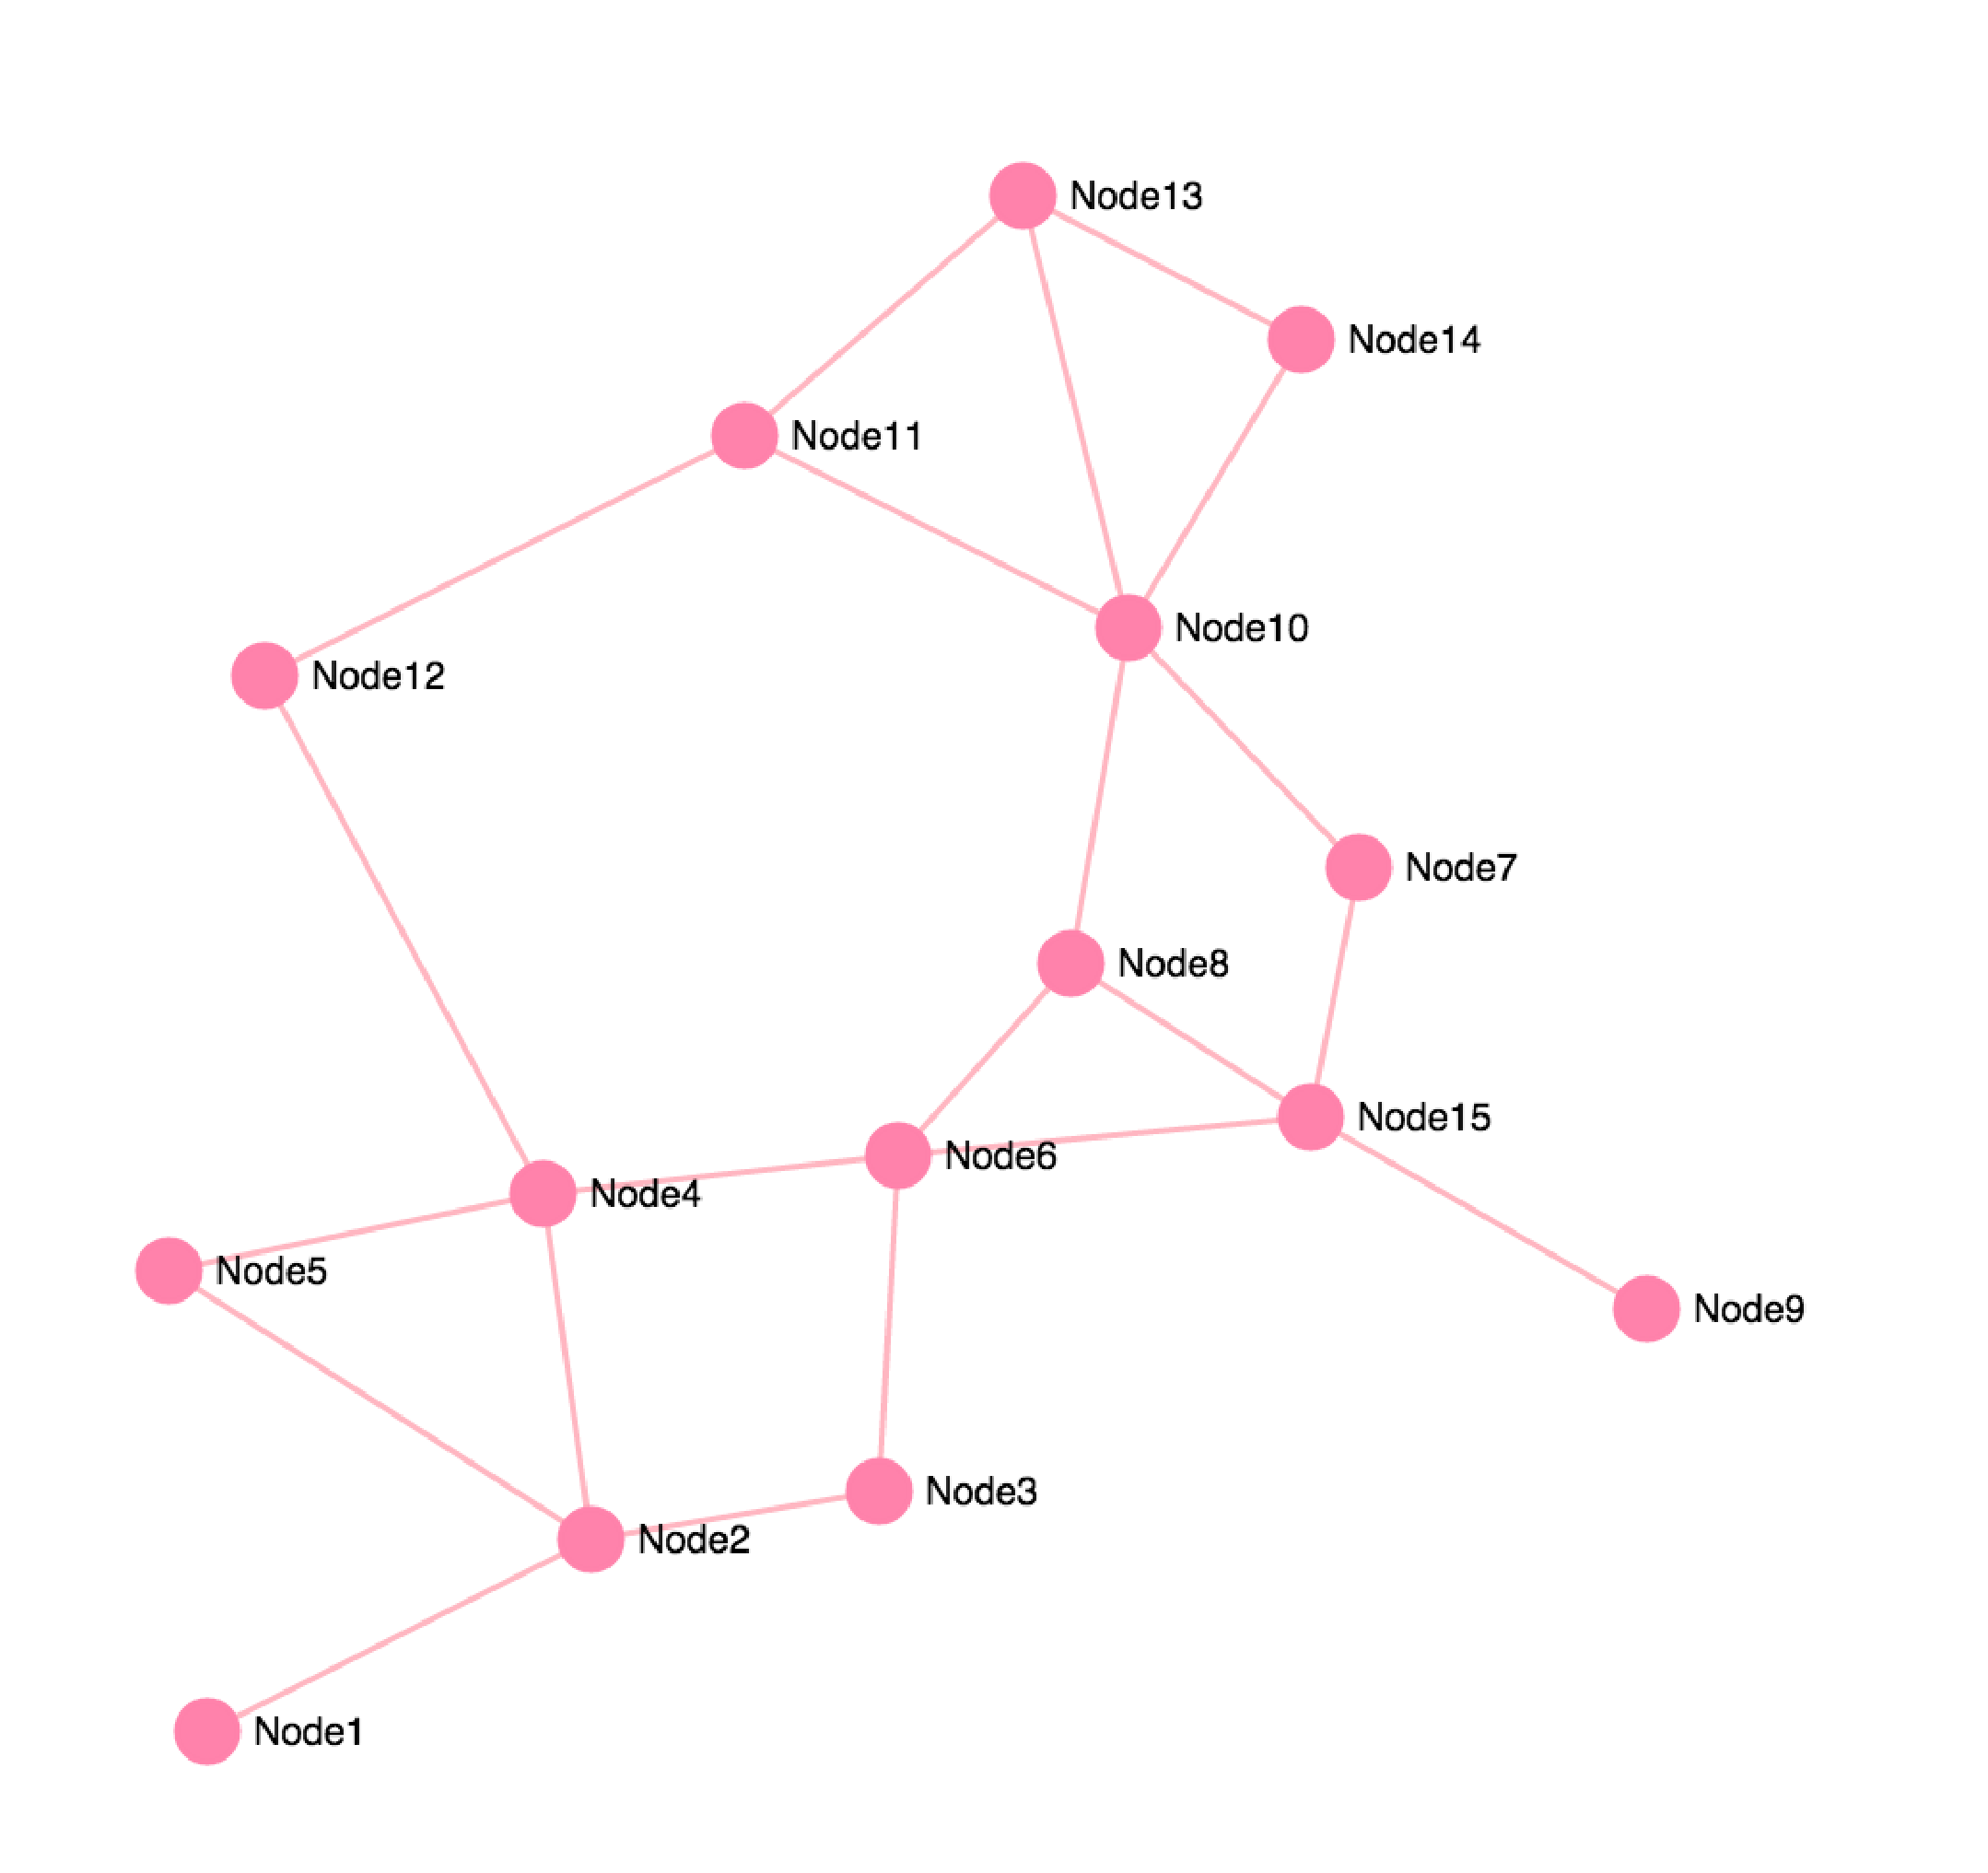
\includegraphics[width=4in]{assets/mandlnetwork_crop.png}
  \end{center}
  \caption[Transit Network]
   {Mandl's Transit Network} 
   The transit network including the 15 nodes and 21 edges. The graph is undirected. \emph{\color{red} TODO: Assumptions that it is undirected} Coordinates are correct based on the MandlCoordinates.txt file from \citep{mumford13}
\end{figure}